\documentclass[11pt,a4paper]{article}
\usepackage[T1]{fontenc}
\usepackage{iftex}
\ifPDFTeX\usepackage[utf8]{inputenc}\fi
\usepackage{lmodern}
\usepackage[margin=25mm]{geometry}
\usepackage{amsmath,amssymb,graphicx,booktabs,microtype}
\usepackage[numbers,sort&compress]{natbib}
\usepackage{xcolor}
\usepackage[colorlinks=true,allcolors=blue!45!black]{hyperref}
\usepackage[font=small,labelfont=bf]{caption}
\graphicspath{{figures/}}
% Generated by scripts/compare_diagrams.py
\newcommand{\NestedPixels}{0.45}
\newcommand{\ConformalPixels}{13.12}
\newcommand{\CosmicPixels}{0.011}
\newcommand{\NullAngle}{51.57}

\title{Comparing Cosmological Diagrams\\[0.4em]\large What do view lines and nested spatial layers add?}
\author{Geometry of Spacetime project}
\date{Research assessment, 27 November 2026}
\begin{document}
\maketitle

\noindent\textbf{Assessment.} The nested-layer representation is useful for
making spatial scale and cosmic-time slices explicit. Its basic polar map
already exists in educational cosmology. It supplies no additional physical
information, and it is less convenient for reading causal relationships
or resolving early epochs. The most defensible role is a companion to a
conformal diagram, with identical events highlighted in both. Whether that
pair improves understanding is an empirical question not answered here.

\section{Existing approaches and the closest precedent}
This is a targeted source comparison, not an exhaustive history or a claim
about the first person to draw a particular map. The following sources were
checked on 27 November 2026.

\begin{description}
\item[Direct polar precedent.] Wright's tutorial uses spatial angle and
scale-factor radius, together with a past light cone, in its
\texttt{omega\_2.gif} diagram \citep{WrightTutorial}. This is the same basic
mapping as ours. The inspected page states that it was last modified on
21 July 2017; that is not an established creation date for the figure.
\item[Matched spacetime views.] Davis and Lineweaver compare three views of
one cosmology in Figure~1: proper distance, comoving distance, and conformal
time \citep{DavisLineweaver2004}. Coordinating different representations
is therefore also established practice. Our Figure~\ref{fig:four} uses our
closed-dust model, rather than reproducing their numerical cosmology.
\item[Causal structure.] Tong explains straight radial null lines in
conformal coordinates and illustrates closed-universe causal diagrams
\citep{TongCosmology}. A Penrose diagram additionally addresses conformal
boundaries; an ordinary finite-window conformal plot is not automatically
a complete Penrose diagram.
\item[Observed history.] Wiltshire's animated light-cone illustration
already relates received light to galaxy histories \citep{WiltshireLightCone}.
Bersanelli's Figure~5 pairs concentric observed epochs with a past-light-cone
sketch \citep{Bersanelli2016}. Those observer-centred shells must be
distinguished from our complete constant-time spatial slices. The visual
comparison does not adopt that article's stronger claims about topology
or a point-like cosmic origin.
\end{description}

\noindent\textbf{Implication for novelty.} Neither polar plotting nor looking
back through cosmic history establishes a new contribution. A possible
contribution would be a demonstrably clearer explanation, a useful linked
implementation, or a separate new physical calculation. Those require
their own evidence.

\clearpage
\section{The same events in four drawings}
To isolate the effect of representation, set the mass perturbation to zero.
All panels use the same closed-dust background and reception event:
\[
 \frac{A}{A_{\max}}=\sin^2(\eta/2),\qquad
 \frac{ct}{A_{\max}}=\frac{\eta-\sin\eta}{2},\qquad
 O:(\eta_o,\chi_o)=(1.8,0).
\]
On the displayed great-circle patch, the two incoming rays obey
$\chi=\pm(\eta_o-\eta)$. The four coordinate pairs are
$(\chi,ct/A_{\max})$, $(A\chi/A_{\max},ct/A_{\max})$,
$(\chi,\eta)$, and $(A/A_o)(\cos\chi,\sin\chi)$.
Here signed $D=A\chi$ is spatial arc separation at the specified epoch,
not luminosity distance or angular-diameter distance.

\begin{figure}[h!]
 \centering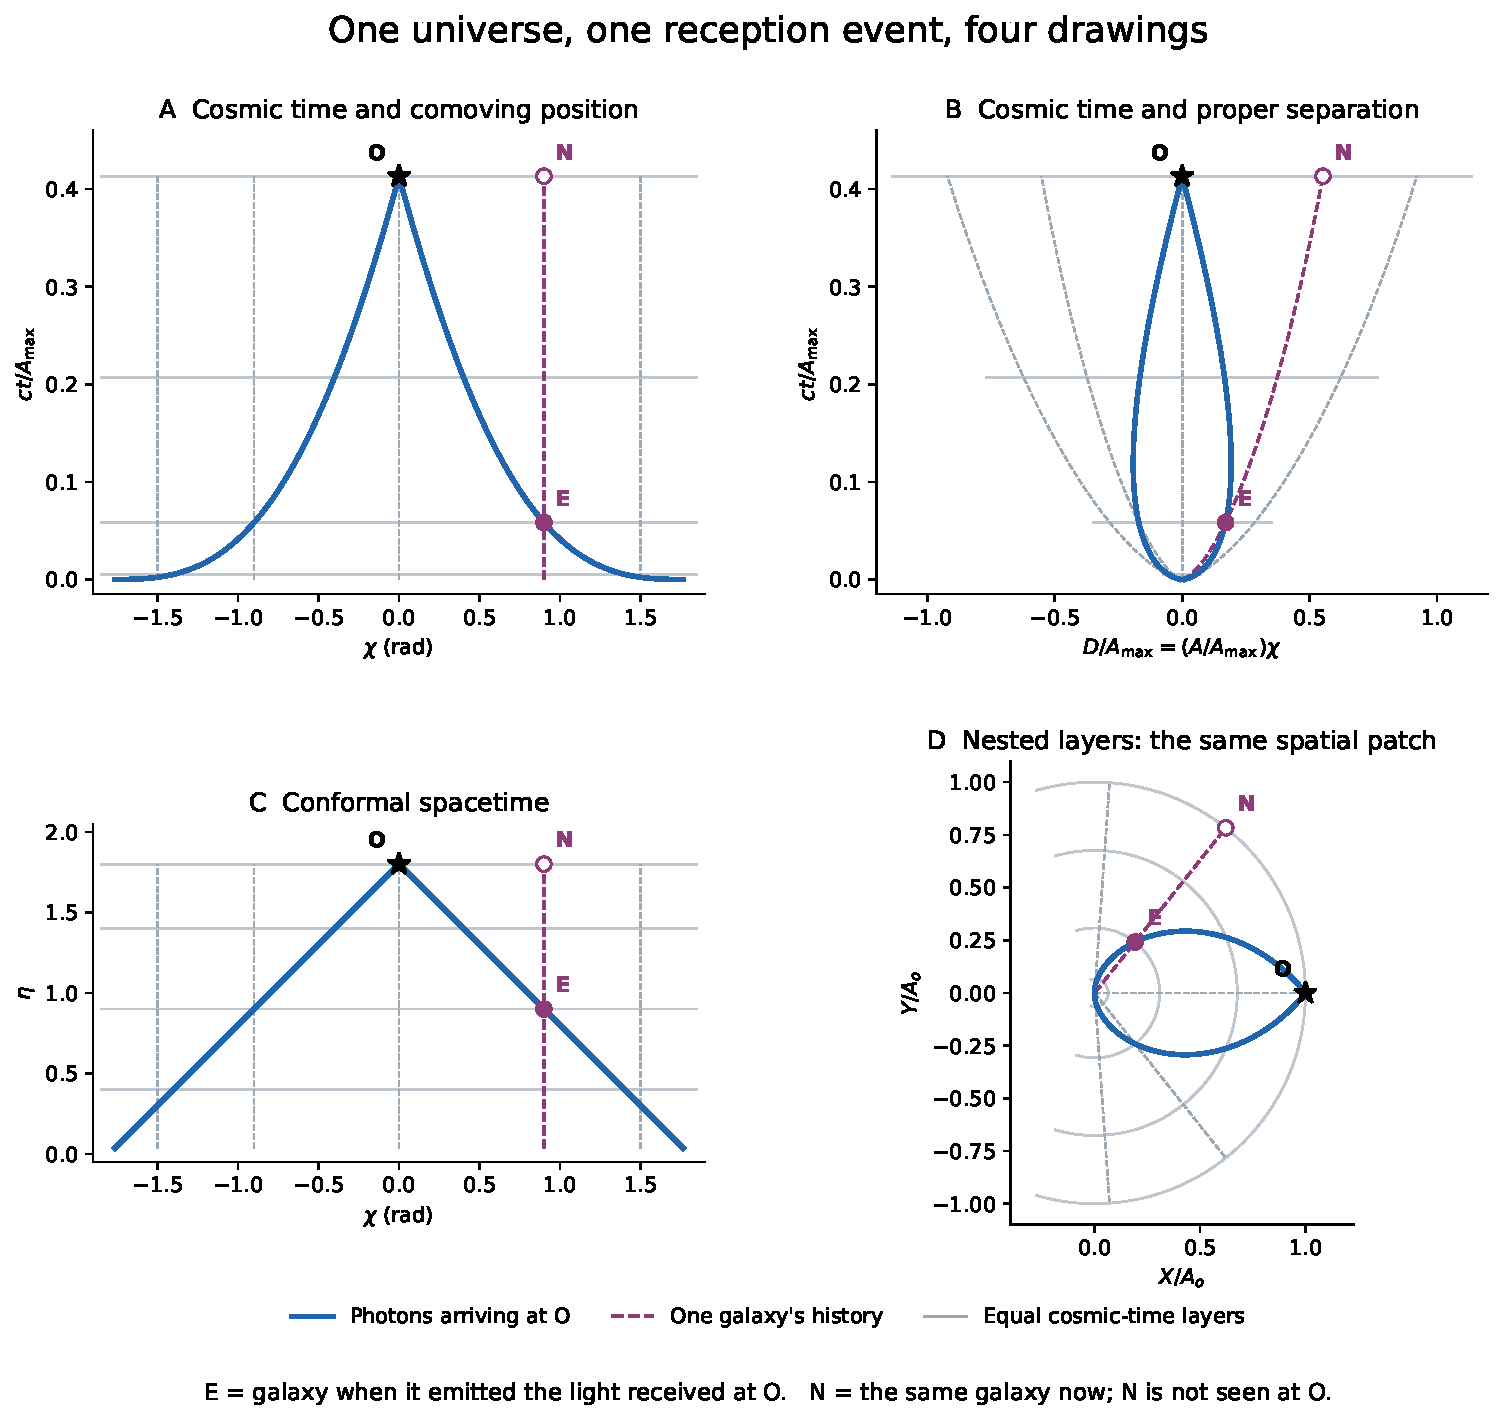
\includegraphics[width=\linewidth]{07-diagram-comparison.pdf}
 \caption{Original calculations, identical events and spatial patch in every
 panel. The emission event is $E=(0.9,0.9)$; $N=(1.8,0.9)$ is the same
 comoving galaxy at reception time. Only $E$ lies on the received light ray.
 Equal axis units in panel C make null lines $45^\circ$. Panels A and B
 use different axis scales. Panel D preserves the chosen spatial scale
 in each circular arc, but its apparent ray curvature is not local lensing:
 there is no localized mass in this comparison.}
 \label{fig:four}
\end{figure}

\noindent Every panel distinguishes $E$ from $N$ once its coordinates are
understood. The nested map adds a visible size change to that distinction;
it does not supply a new emission event, travel time, or causal connection.

\clearpage
\section{A whole time slice is not the visible universe}
For the unperturbed closed model, write a spatial slice as
$\mathbf X=A(\eta)\mathbf n$, with $\mathbf n\in S^3$. An observer at
$(\eta_o,\mathbf n_o)$ sees, at epoch $\eta$, the direct light-cone subset
\[
 \mathcal V_\eta=
 \{\mathbf n\in S^3:\arccos(\mathbf n\cdot\mathbf n_o)=\eta_o-\eta\},
 \qquad 0<\eta_o-\eta<\pi.
\]
This subset is a two-sphere inside the three-sphere. A drawing that shows
an entire nested layer as visible would be misleading. Figure~\ref{fig:subset}
marks the distinction explicitly, using lower-dimensional sections.

\begin{figure}[h!]
 \centering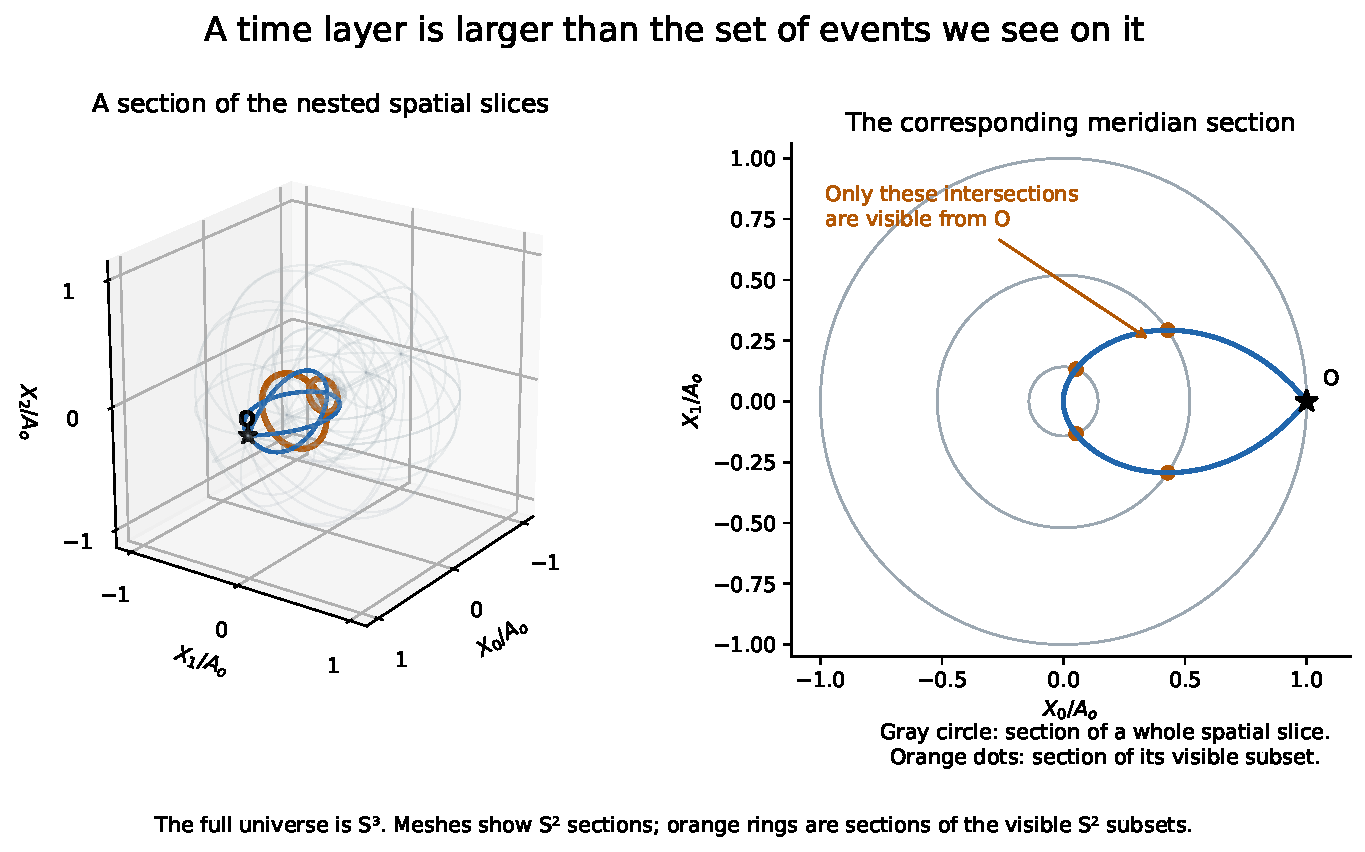
\includegraphics[width=\linewidth]{08-slices-and-visible-subsets.pdf}
 \caption{Gray meshes are $S^2$ sections of the full $S^3$ spatial slices.
 Orange circles are the intersections of those sections with the visible
 $S^2$ subsets at $\eta=0.6$ and $1.2$; they are not complete spatial
 universes. Blue curves are sample rays. The right-hand meridian section
 reduces those orange circles to pairs of points. Projection can overlap
 distinct features in the three-dimensional view.}
 \label{fig:subset}
\end{figure}

\subsection*{What this version might help explain}
The nested picture can explicitly show a spatial slice, the visible
subset of that slice, and a light path crossing slices in one construction.
It also makes increasing spatial arc lengths at fixed angular separation
visible. These are plausible explanatory benefits, not measured learning
outcomes. Conventional light-cone diagrams and expanding-balloon animations
can also convey them.

\subsection*{What the drawing must not imply}
The origin of the drawing is not a location on a spatial slice. Looking
back toward smaller radii does not identify a telescope direction toward a
physical centre. Rotating the homogeneous spatial coordinates moves the
observer without changing the physics. The angle used to locate an event
around a drawn circle is not the source's angular position on the sky.
Moving toward an earlier slice is tracing a history, not a possible
future-directed journey into the past.

\clearpage
\section{Mathematical limits that can already be tested}
\begin{figure}[h!]
 \centering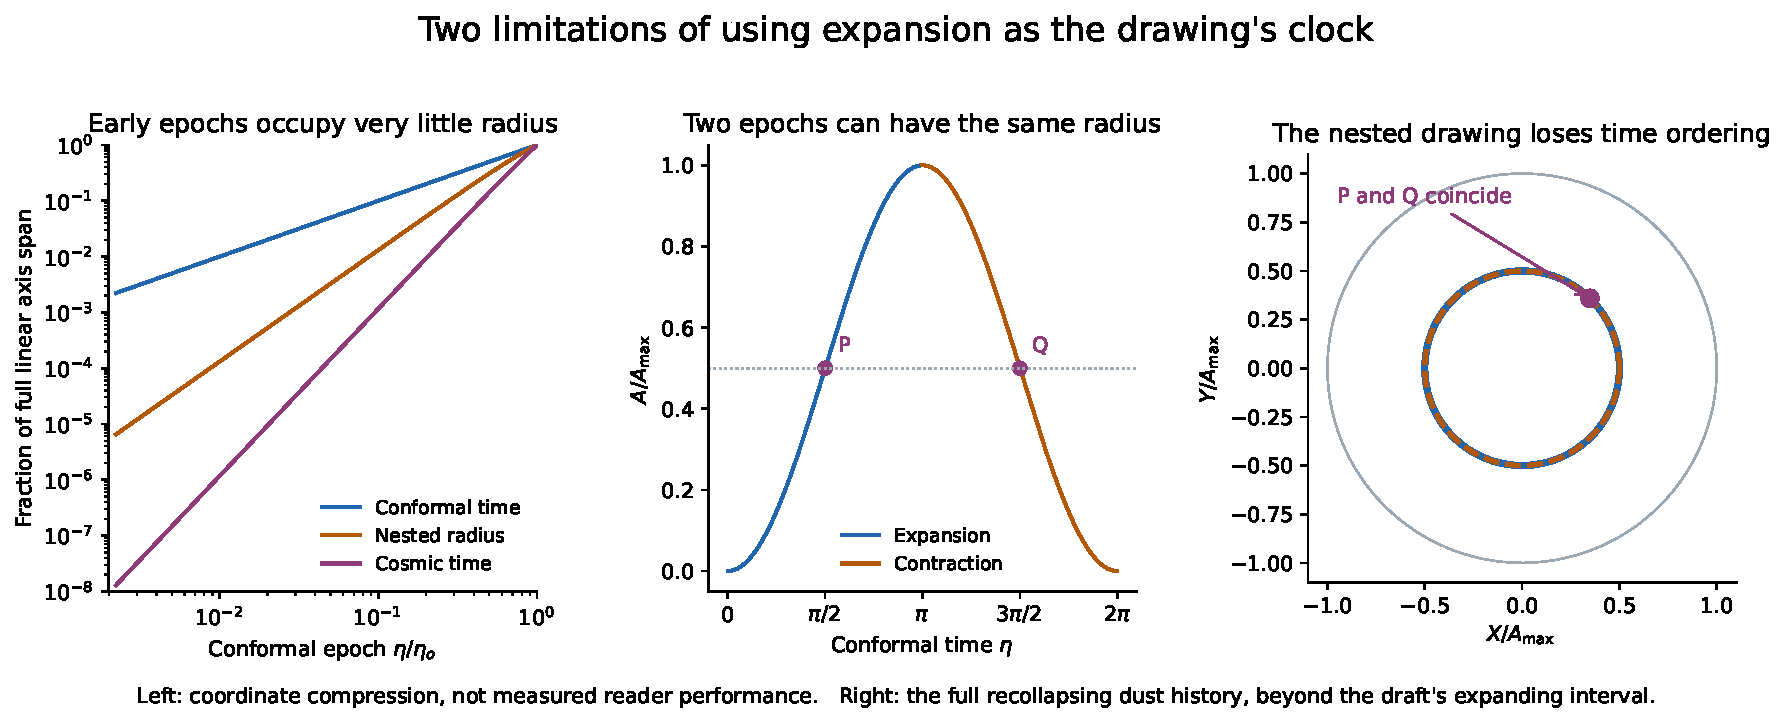
\includegraphics[width=\linewidth]{09-diagram-stress-tests.pdf}
 \caption{Coordinate compression and loss of injectivity. The last two
 panels deliberately extend the homogeneous dust solution through
 recollapse; the weak-field paper restricts its calculation to expansion.}
 \label{fig:limits}
\end{figure}

\paragraph{Early epochs become small.}
Consider the illustrative epoch $1+z=A_o/A=1100$ in this dust model.
It is not a calculation of recombination. For a 500-pixel linear span from
the formal initial boundary to reception, its coordinate offset is:
\begin{center}
\begin{tabular}{lrr}
\toprule
Coordinate & Normalized value & Pixel offset\\
\midrule
Nested radius & $1/1100$ & $\NestedPixels$\\
Conformal time & $\eta/\eta_o$ & $\ConformalPixels$\\
Cosmic time & $t/t_o$ & $\CosmicPixels$\\
\bottomrule
\end{tabular}
\end{center}
The comparison fixes each coordinate's full linear span; it is not a
reader-performance score. The nested radial coordinate resolves early
epochs better than cosmic time in this example, but much less well than
conformal time. A zoom or nonlinear radial stretch can improve visibility,
at the cost of a different scale interpretation.

\paragraph{Radius is not a global clock.}
For $R=A/A_o$, the local Jacobian of $(\eta,\chi)\mapsto(X/A_o,Y/A_o)$ is
\[
 J=R R',\qquad R'=R\cot(\eta/2).
\]
At maximum expansion $\eta=\pi$, $J=0$. The two events
$(\pi/2,0.8)$ and $(3\pi/2,0.8)$ have different cosmic times but the same
drawn position. To include both eras, add a branch/time coordinate or
separate panels. A static interval is another case where scale-factor
radius cannot label time. The usual angular coordinate seam is a separate
issue and can be handled by patches.

\paragraph{Ray slopes and shapes depend on the drawing.}
For a background radial photon on the expanding branch, the acute angle
$\beta$ to the radial time direction satisfies
\[
 \tan\beta=\frac{R|d\chi/d\eta|}{R'}=\tan(\eta/2).
\]
It is $\NullAngle^\circ$ at our reception epoch; there is no universal
$45^\circ$ null rule in the nested drawing. Curved rays there are not
evidence for a local gravitational lens. Physical deflections require
observer frames and matched sources, as in the main paper.

\clearpage
\section{Which representation serves which question?}
The following is an analytical assessment of what is explicitly encoded,
not a measured ranking of educational effectiveness.

\begin{center}\small
\begin{tabular}{@{}p{.25\linewidth}p{.33\linewidth}p{.34\linewidth}@{}}
\toprule
Question & Most direct representation & Role of nested layers\\
\midrule
{\raggedright Which emission reaches this observer?\par} & {\raggedright Conformal null lines and galaxy worldlines.\par} & {\raggedright Same intersections, with changing scale visible.\par}\\[4pt]
{\raggedright Where is the galaxy now versus when seen?\par} & {\raggedright Any labelled spacetime map; $E$ and $N$ in Fig.~\ref{fig:four}.\par} & {\raggedright Clear separate layers if both events are marked.\par}\\[4pt]
{\raggedright How do spatial separations grow?\par} & {\raggedright Proper-distance plot or expanding spatial-slice animation.\par} & {\raggedright Arc lengths scale with $A$ directly.\par}\\[4pt]
{\raggedright What can causally influence what?\par} & {\raggedright Conformal diagram; an appropriate global conformal/Penrose diagram for boundaries.\par} & {\raggedright Variable null directions need an additional legend or construction.\par}\\[4pt]
{\raggedright What does an early epoch look like across the sky?\par} & {\raggedright Observer-centred past-cone intersection with that epoch.\par} & {\raggedright Must highlight the visible subset, not the entire slice.\par}\\[4pt]
{\raggedright Does a local mass deflect light?\par} & {\raggedright Matched observer-frame angles and lensing observables.\par} & {\raggedright Ray appearance alone is insufficient.\par}\\[4pt]
{\raggedright Does the map span contraction as well?\par} & {\raggedright Monotonic cosmic/conformal time coordinate.\par} & {\raggedright Scale-factor radius folds unless branch information is added.\par}\\
\bottomrule
\end{tabular}
\end{center}

\paragraph{Working recommendation.}
Keep a conformal view as the reference and offer the nested view alongside
it, with linked highlights for the same event and worldline. State the
dimensions suppressed, show the observer on the current slice, and mark
only the relevant light-cone intersections as observed. Use a numerical
readout for cosmic time, redshift, and proper separation rather than
asking readers to infer all three from the geometry of the drawing.

The new local-mass calculation remains separate from this assessment.
Spatial deformation, elapsed proper time, and observational light paths
have different meanings; the existing weak-field result already requires
separate drawing conventions for deformation and history. A diagram that
needs these distinctions is still usable, but should not be presented as
a single literal picture from which gravity follows.

\paragraph{Evidence status.}
The source overlap, coordinate equivalence, null slopes, compression, and
time-folding are established for the specified maps. Increased clarity,
reduced confusion, and greater learning are hypotheses. No participants
were recruited or simulated, and no educational result is reported.

\clearpage
\section{A reader study to test the remaining claim}
\textbf{Proposed protocol; not yet run.} First pilot the questions and
instructions for ambiguity. A small convenience pilot can improve the
materials, but cannot establish a general learning benefit. Set sample
size, scoring, and decision criteria before a subsequent comparison.

\paragraph{Fair comparison.}
Randomly assign readers to (A) conformal plus proper-distance views, or
(B) conformal plus nested-layer views. Keep the total display area,
cosmological parameters, event labels, colours, explanation length, and
interaction controls comparable. Giving only B a second panel or an
animation would confound the test. Record prior relativity knowledge;
use a pre-test and unfamiliar transfer examples. A nested-only condition
could be a separate exploratory comparison.

\paragraph{Six tasks and an explicit answer key.}
Score each task against a predefined rubric, with wording refined in the
pilot. Assess explanations as well as clicking the right point.
\begin{enumerate}
\item Identify which event on the marked galaxy's history is visible at
$O$. \emph{Key: $E$, not $N$.}
\item Identify the event on that galaxy at the same background cosmic
time as reception. \emph{Key: $N$, on $O$'s time slice.}
\item Mark what is visible at one earlier epoch.
\emph{Key: the light-cone intersection, not the entire spatial slice.}
\item Decide whether the middle of the polar drawing is a place that
could be reached by travelling along a present spatial slice.
\emph{Key: no; the drawing's origin is not a location on that slice.}
\item Decide whether the curved blue path in Fig.~\ref{fig:four} proves
deflection by a localized mass. \emph{Key: no; this model has no mass
perturbation, and path shape changes with the coordinate map.}
\item On a new observer position or reception epoch, identify another
emission and explain the same-time/seen-time distinction.
\emph{Key: use the new past cone and the marked time slice, not memorized
positions from the training figure.}
\end{enumerate}

\paragraph{What to measure.}
Choose transfer-task accuracy as the primary outcome. Record task time
and confidence separately, and report centre/lensing misconceptions
explicitly rather than hiding them in an average. Use uncertainty intervals
appropriate to the study design. Do not replace reader data with the
author's or an AI system's ratings of how intuitive the plots look.

\paragraph{Decision.}
Retain the nested view as an educational contribution if it improves the
target distinctions without an unacceptable increase in the critical
misconceptions. If performance is similar, its value may be preference
or engagement. If it worsens understanding, revise or remove it from the
main explanation. The present comparison justifies testing the paired
view; it does not predict that it will win.

\paragraph{Reproducibility.}
\texttt{make comparison} regenerates the figures, CSV event coordinates,
JSON diagnostics, and this PDF. Three additional tests check event recovery,
the recollapse counterexample, and the visible-subset geometry. The main
calculation's tests remain separate. The source figures reviewed for this
assessment are linked in the bibliography; no third-party artwork is
reproduced in these generated figures.

\clearpage
\bibliographystyle{plainnat}
\bibliography{references}
\end{document}
